%%\documentclass[aspectratio=1610]{beamer}
\documentclass[xcolor=dvipsnames,hyperref={colorlinks,urlcolor=magenta}]{beamer}
%
%%%%%%%%%%%%%%%%%%%%%%%%%%%%%%%%%%%%
%% Common preamble
%%%%%%%%%%%%%%%%%%%%%%%%%%%%%%%%%%%%
% PAGE
%% \usepackage{fullpage}
% FONTS
\usepackage{lmodern} % enhanced version of computer modern
\usepackage[T1]{fontenc} % for hyphenated characters
%% \usepackage{gillius2}
%% \renewcommand{\familydefault}{\sfdefault}
\usepackage{amssymb}
\usepackage{mathtools} % contains amsmath which comes with align
\usepackage{amsthm}
%%\usepackage{enumitem}
\usepackage{microtype} % some compression
%%%%%%%%%%%%%%%%%%%%%%%%%%%%%%%%%%%%
\usepackage{subfig}
\usepackage{tikz}
\usetikzlibrary{spy,shadows,arrows,shapes,positioning,calc,backgrounds,fit,automata}
\newcommand{\score}{\text{score}}

\definecolor{myblue}{HTML}{C5E0DC}
\definecolor{vtblue}{HTML}{557082}
\definecolor{hokie}{HTML}{660000}
\definecolor{hokieRed}{HTML}{980000}

\definecolor{col1}{HTML}{D53E4F}
\definecolor{col2}{HTML}{F46D43}
\definecolor{col3}{HTML}{FDAE61}
\definecolor{col4}{HTML}{FEE08B}
\definecolor{col5}{HTML}{E6F598}
\definecolor{col6}{HTML}{ABDDA4}
\definecolor{col7}{HTML}{66C2A5}
\definecolor{col8}{HTML}{3288BD}

\newcommand{\dunder}[1]{\underline{\underline{#1}}}
\newcommand{\dmax}{d_{\max}}
\newcommand{\cost}{\text{cost}}
%\newcommand{\comment}[1]{{\color{red}#1}}
\newcommand{\wmin}{w_{\min}}
\newcommand{\copt}{C_{\text{OPT}}}
\newcommand{\TikZ}{Ti\textit{k}Z\xspace}
\newcommand{\tuta}{\emph{T. absoluta}}
\newcommand{\prempt}{\textsc{PREMpT}}

%%
\title[]{Learning the Behavior of a Dynamical System Via a ``20 Questions" Approach}
\date[Feb. 6, 2018]{February 6, 2018}
\author[A.~Adiga]{\textbf{Abhijin Adiga}, Chris~J.~Kuhlman,
Madhav~V.~Marathe, S.~S.~Ravi, Daniel~J.~Rosenkrantz and Richard~E.~Stearns}
\institute[]{\centering
    \mbox{}\hspace{.9cm}\raisebox{.6cm}{\includegraphics[width=3.5cm]{figs/ndssl_logo.png}}\hspace*{.4cm}~\raisebox{.0cm}{\includegraphics[width=4cm]{figs/bivt_logo.pdf}}~\raisebox{.3cm}{\includegraphics[width=2.2cm]{figs/albany_logo.png}}
}

\usetheme{Boadilla}
\usecolortheme{seagull}
\setbeamercolor{structure}{fg=vtblue}
\setbeamercolor{alerted text}{fg=hokieRed}
\setbeamerfont{alerted text}{series=\mdseries}
%% This ``scales'' the font. Don't extend too much beyond 128x96
%% Uncomment the next line for default sizes:
\geometry{paperwidth=140mm,paperheight=96mm}
%% \setbeamercolor{block title}{use=structure,fg=white,bg=black!75!white}
%% \setbeamercolor{block body}{use=structure,fg=black,bg=black!10!white}
%%
%% ----------------------------------------------------------------------
%%
\begin{document}
%%
%% %% ----------------------------------------------------------------------
%% \begin{frame}
%% \titlepage
%% \end{frame}
%% %% ----------------------------------------------------------------------
\newcommand{\parnode}[1]{\parbox{3cm}{\centering #1}}
\begin{frame}
    \frametitle{Outline}
\begin{itemize}
    \item Inferring propagation models over networks
\end{itemize}
%% ----------------------------------------------------------------------
\centering
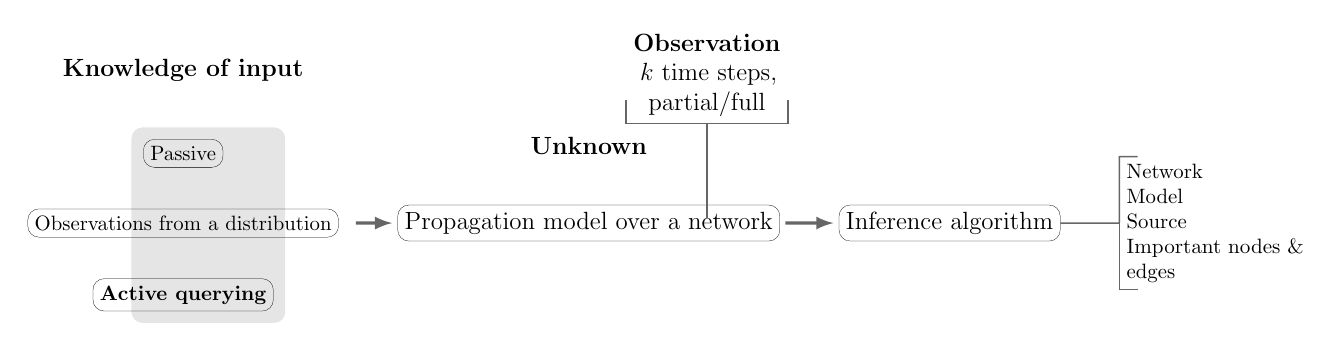
\begin{tikzpicture}
[scale=.75,auto,transform shape,
edge/.style={black!60,>=latex, shorten >=2pt, shorten <=2pt, line width=.4mm},
block/.style={draw=black,ultra thin,rounded corners}]
%%
\node[block] (passive) {\parnode{Passive}};
%%
\node (random) [block,below=of passive,shift={(0,.3)}]{\parnode{Observations from a
distribution}};
%%
\node (act) [block, below=of random,shift={(0,.3)}] {\parnode{\bf Active querying}};
%%
\node [above of=passive,shift={(0,.4)},font=\large] {\parnode{\bf Knowledge of input}};
%%
\begin{pgfonlayer}{background}
\draw[rounded corners,fill=black!10,draw=none] ($(passive.north
west)+(-.2,.2)$) rectangle ($(act.south east)+(.2,-.2)$);
\end{pgfonlayer}
%%
\node (gds) [block,right=of random,font=\large] {\parnode{Propagation model over a
network}};
\node [above of=gds,shift={(0,.3)},font=\large] {\parnode{\bf Unknown}};
\node (obs) [above of=gds,shift={(2,1.5)},font=\large]
{\parbox{2.5cm}{\centering{\bf
Observation}\\$k$ time steps, partial/full}};
\node (inf) [block,right=of gds,font=\large] {\parnode{Inference algorithm}};
\node (result) [right=of inf] {\parbox{3cm}{Network \\ Model \\
Source \\ Important nodes \& edges}};
%%
\draw[edge,->] ($(random.east)+(.2,0)$) -- (gds);
\draw[edge,->] (gds.east) -- (inf);
\draw [edge,line width=.2mm] (inf.east) -- (result) -|
(result.north west) -- +(.4,0);
\draw [edge,line width=.2mm] (result) -| (result.south west) -- +(.4,0);
\draw [black!60,line width=.2mm] ($(obs.south)+(0,-1.6)$) -- (obs.south) --
(obs.south west) -- +(0,.4);
\draw [black!60,line width=.2mm] (obs.south) -- (obs.south east) -- +(0,.4);
\end{tikzpicture}
%% ----------------------------------------------------------------------
\begin{itemize}
    \item Accuracy of inference: exact or approximate
    \item Knowledge: partial or full
\end{itemize}
%% \alert{Not at all comprehensive}
\end{frame}
%% ----------------------------------------------------------------------
\begin{frame}
\frametitle{Problem: Inferring propagation models by active querying}
\centering
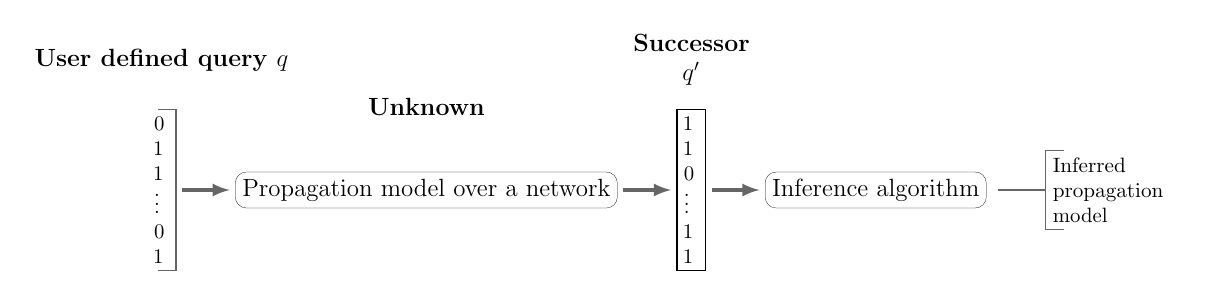
\begin{tikzpicture}
[scale=.75,auto,transform shape,
edge/.style={black!60,>=latex, shorten >=2pt, shorten <=2pt, line width=.4mm},
block/.style={draw=black,ultra thin,rounded corners}]
%%
\node[] (q) {\parbox{.25cm}{0\\1\\1\\$\vdots$\\0\\1}};
%%
\node [above of=q,shift={(0,1.2)},font=\large] {\parnode{\bf User defined
query~$q$}};
\node (gds) [block,right=of q,font=\large] {\parnode{Propagation model over a
network}};
\node [above of=gds,shift={(0,.4)},font=\large] {\parnode{\bf Unknown}};
\draw[edge,->] (q.east) -- (gds);
\draw [black!60,line width=.2mm] (q.east) |- (q.north east) -- +(-.3,0);
\draw [black!60,line width=.2mm] (q.east) |- (q.south east) -- +(-.3,0);
\node[right=of gds,draw] (qp) {\parbox{.25cm}{1\\1\\0\\$\vdots$\\1\\1}};
%%
\node [above of=qp,shift={(0,1.2)},font=\large] {\parbox{2cm}{\centering\bf Successor 
$q'$}};
\node (inf) [block,right=of qp,font=\large] {\parnode{Inference algorithm}};
\node (result) [right=of inf] {\parbox{2cm}{Inferred propagation model}};
%%
\draw[edge,->] (gds.east) -- (qp);
\draw[edge,->] (qp) -- (inf);
\draw [edge,line width=.2mm] ($(inf.east)+(.2,0)$) -- (result) -|
(result.north west) -- +(.4,0);
\draw [edge,line width=.2mm] (result) -| (result.south west) -- +(.4,0);
\end{tikzpicture}
   \begin{itemize}
       \item User knows:
       \begin{itemize}
           \item Network (undirected, unweighted)
           \item Concept class
           \begin{itemize}
               \item threshold functions
               \item symmetric local functions
       \end{itemize}
       \end{itemize}
       \item Exact inference
   \end{itemize}
   \alert{Sample complexity: How many queries are sufficient to infer the dynamical system?}
   %% \includegraphics[width=.3\textwidth]{figs/query_gds.jpg}
\end{frame}
%% ----------------------------------------------------------------------
%% \begin{frame}
%%     \frametitle{Motivation and previous work}
%% \begin{itemize}
%%     \item Threshold models have wide-spread application in modeling
%%     protests, information diffusion (e.g., word of mouth, social media),
%%     adoption of practices (e.g., contraception, innovation), transmission
%%     of emotions.
%%     \item Social science network experiments (Centola 2010)
%%     \item Serves as a baseline for more realistic inference problems
%%        \item General inference: (Gonz\'{a}lez-Bail\'{o}n~et~al.~2011; Romero,~Meeder,~and~Kleinberg~2011) present methods to infer thresholds from social media data.
%%        \item Active inference: (Kleinberg, Mullainathan and Ugander 2017)
%%        for the choice set problem
%%    \end{itemize}
%% \end{frame}
%% ----------------------------------------------------------------------
\begin{frame}
    \frametitle{Threshold propagation model}
    \framesubtitle{... and symmetric vertex functions}
   \begin{itemize}
       \item Closed neighborhood of a vertex~$v$: $N[v]$
       \item Every node is associated with a threshold: $t(v)$
   \end{itemize}
   \[
       q_{i+1}(v)=\begin{cases}
           1, & \sum_{v'\in N[v]}q_i(v')\ge t(v) \\
           0, & \text{otherwise}
       \end{cases}
   \]
\centering
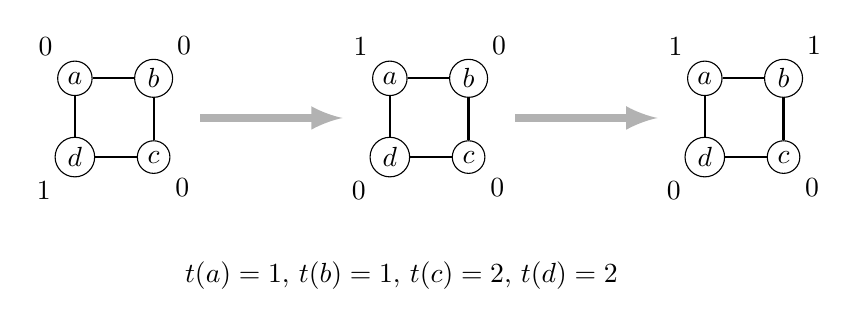
\begin{tikzpicture}
[node distance=1cm,
vertex/.style={shape=circle,draw=black,inner sep=2pt},
thickedge/.style={draw=Gray!60,>=latex, shorten >=.0pt, shorten <=.0pt, 
line width=1mm},
myedge/.style={thick}]
%%
\node[anchor=west] at (1.5,-2.5) {$t(a)=1$, $t(b)=1$, $t(c)=2$, $t(d)=2$};
%%
\begin{scope}[anchor=west,local bounding box=t1]
\node (a) [vertex,label=above left:$0$] at (0,0) {$a$};
\node (b) [vertex,right of=a,label=above right:$0$] {$b$};
\node (c) [vertex,below of=b,label=below right:$0$] {$c$};
\node (d) [vertex,below of=a,label=below left:$1$] {$d$};
\draw[myedge] (a) -- (b) -- (c) -- (d) -- (a);
\end{scope}
%%
\begin{scope}[anchor=west,shift={(4,0)},local bounding box=t2]
\node (a) [vertex,label=above left:$1$] at (0,0) {$a$};
\node (b) [vertex,right of=a,label=above right:$0$] {$b$};
\node (c) [vertex,below of=b,label=below right:$0$] {$c$};
\node (d) [vertex,below of=a,label=below left:$0$] {$d$};
\draw[myedge] (a) -- (b) -- (c) -- (d) -- (a);
\end{scope}
%%
\begin{scope}[anchor=west,local bounding box=t3,,shift={(8,0)}]
\node (a) [vertex,label=above left:$1$] at (0,0) {$a$};
\node (b) [vertex,right of=a,label=above right:$1$] {$b$};
\node (c) [vertex,below of=b,label=below right:$0$] {$c$};
\node (d) [vertex,below of=a,label=below left:$0$] {$d$};
\draw[myedge] (a) -- (b) -- (c) -- (d) -- (a);
\end{scope}
\draw[thickedge,->] (t1) -- (t2);
\draw[thickedge,->] (t2) -- (t3);
%%
\end{tikzpicture}
\begin{itemize}
    \item Symmetric vertex functions: State depends only on number of
    neighbors in state~$1$.
\end{itemize}
\end{frame}
%% ----------------------------------------------------------------------
\begin{frame}
    \frametitle{Query models}
    \framesubtitle{Batch and adaptive modes}
\centering
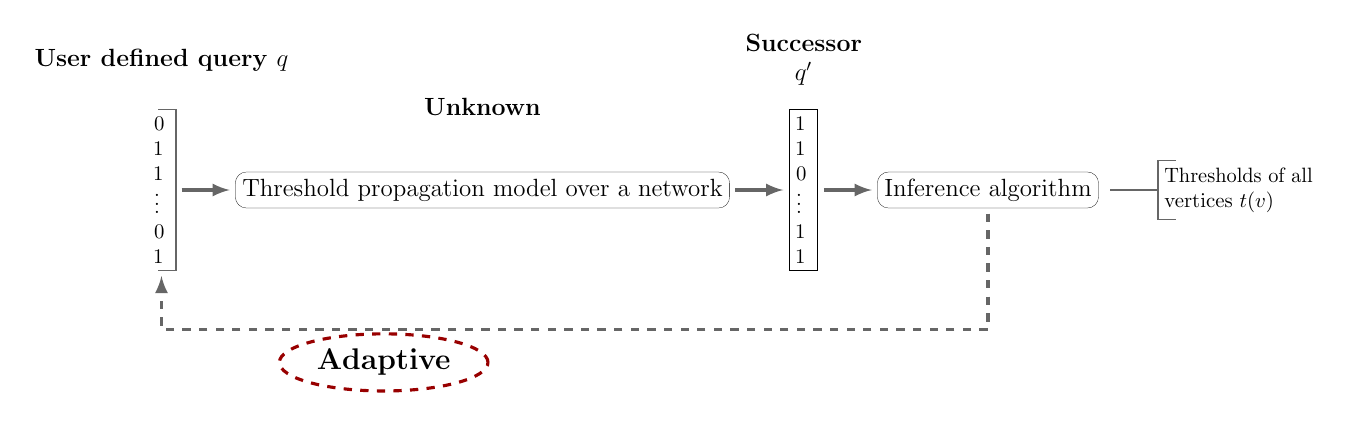
\begin{tikzpicture}
[scale=.75,auto,transform shape,
edge/.style={black!60,>=latex, shorten >=2pt, shorten <=2pt, line width=.4mm},
block/.style={draw=black,ultra thin,rounded corners}]
%%
\node[] (q) {\parbox{.25cm}{0\\1\\1\\$\vdots$\\0\\1}};
%%
\node [above of=q,shift={(0,1.2)},font=\large] {\parnode{\bf User defined
query~$q$}};
\node (gds) [block,right=of q,font=\large] {\parnode{Threshold propagation model over a
network}};
\node [above of=gds,shift={(0,.4)},font=\large] {\parnode{\bf Unknown}};
\draw[edge,->] (q.east) -- (gds);
\draw [black!60,line width=.2mm] (q.east) |- (q.north east) -- +(-.3,0);
\draw [black!60,line width=.2mm] (q.east) |- (q.south east) -- +(-.3,0);
\node[right=of gds,draw] (qp) {\parbox{.25cm}{1\\1\\0\\$\vdots$\\1\\1}};
%%
\node [above of=qp,shift={(0,1.2)},font=\large] {\parbox{2cm}{\centering\bf Successor 
$q'$}};
\node (inf) [block,right=of qp,font=\large] {\parnode{Inference algorithm}};
\node (result) [right=of inf] {\parbox{2.5cm}{Thresholds of all vertices
$t(v)$}};
%%
\draw[edge,->] (gds.east) -- (qp);
\draw[edge,->] (qp) -- (inf);
\draw [edge,line width=.2mm] ($(inf.east)+(.2,0)$) -- (result) -|
(result.north west) -- +(.4,0);
\draw [edge,line width=.2mm] (result) -| (result.south west) -- +(.4,0);
\draw [edge,dashed,->] (inf) |- ($(q.south)+(0,-1)$)
node[below right,black,font=\Large,shift={(2.5,-.2)},ellipse,draw=hokieRed] {\bf Adaptive} -- (q);
\end{tikzpicture}
\begin{itemize}
    \item Batch: queries must be submitted at once.
    \item Adaptive: a query can be submitted after observing answers
    to previous queries (\alert{``Twenty questions'' game}).
\end{itemize}
\end{frame}
%% ----------------------------------------------------------------------
\begin{frame}
\frametitle{Inferring the threshold of a single vertex}
\centering
\begin{tikzpicture}[scale=.75,myedge/.style={thick,dedge},
vertex/.style={shape=circle,inner sep=.1pt,draw},
source/.style={shape=circle,fill=myRed,draw=myRed,inner sep=2pt}]
\node (v) [vertex,inner sep=1pt] at (0,0) {$v$};
\def \n {5}
\def \rad {1.25cm}
\foreach \x in {1,...,\n}
\draw node(u\x)[vertex] at ({360/\n * -\x}:\rad) {\small $u_\x$};
\foreach \x in {1,...,\n}
\draw (v)--(u\x);
\node at (5,0) {\parbox{4cm}{Threshold $t(v)=5$ \\ Degree $d(v)=5$}};
\node at (-.5,-5.5) [label=above:Batch mode] {\includegraphics[height=4.5cm]{figs/batch.pdf}};
\node at (7.5,-5.5) [label=above:Adaptive mode] {\includegraphics[height=4.5cm]{figs/adaptive.pdf}};
\end{tikzpicture}
%%\includegraphics[width=.8\textwidth]{figs/query_function.jpg}
\end{frame}
%% ----------------------------------------------------------------------
%% \begin{frame}
%%     \frametitle{Extending to the network setting}
%%     \begin{itemize}
%%    \item Inferring all thresholds by naive approach: $n\times\dmax$ for batch
%%    mode and $n\log \dmax$ for adaptive, where~$\dmax$ is the max. degree.
%%    \item Can we do better?
%%    \item Is it close to the single vertex case?
%%    \begin{itemize}
%%        \item A clique of size~$n$ with distinct thresholds requires $n$ queries
%%    even in the adaptive mode!
%%    \end{itemize}
%%     \end{itemize}
%% \end{frame}
%% ----------------------------------------------------------------------
%% \begin{frame}
%%    \frametitle{Results}
%%    \begin{itemize}
%%       \item Upper and lower bounds on optimal query set size for inferring threshold
%%       systems exactly for a dynamical system with
%%       \begin{itemize}
%%          \item symmetric local functions in batch mode 
%%          \item threshold model in adaptive mode
%%       \end{itemize}
%%       \item Algorithms for inference and their evaluation on a number of synthetic and real-world
%%       networks
%%       \item Query compaction: Given a set of queries, can we identify
%%       redundant queries and remove them to make the query set more compact?
%%    \end{itemize}
%%    Key concepts
%%    \begin{itemize}
%%        \item Distance-two vertex coloring of graphs
%%        \item Probabilistic methods
%%        \item Set cover
%%       %% \item {We show that very few queries are required to infer
%%       %%    a threshold/symmetric dynamical system.}
%%    \end{itemize}
%% \end{frame}
%% ----------------------------------------------------------------------
%% \begin{frame}
%%    \frametitle{Batch querying results}
%%    \begin{itemize}
%%    \item \alert{Applies even to symmetric local functions}
%%       \item Lower bound: $\dmax+2$
%%       \item Upper bound: based on distance-two coloring
%%       \item Query set based on random queries
%%    \end{itemize}
%% \end{frame}
%% ----------------------------------------------------------------------
%% \begin{frame}
%%    \frametitle{Upper bound}
%%    {\centering
%%    \begin{tikzpicture}
%%        \node {\includegraphics[width=.8\textwidth]{figs/gsquared_wiki.pdf}};
%%        \node[font=\small] at (5,-2) {\parbox{2cm}{Courtesy wikipedia}};
%%        \node[font=\Large] at (-5.3,.7) {$v$};
%%        \node[font=\Large] at (-2.7,1.3) {$u_1$};
%%        \node[font=\Large] at (-1,-1.3) {$u_2$};
%%    \end{tikzpicture}
%%    }
%% 
%%    \structure{Sufficient condition:} If two nodes are apart by a
%%    distance~$\ge3$, then, they can be queried simultaneously.
%% \end{frame}
%% %% ----------------------------------------------------------------------
%% \begin{frame}
%%    \frametitle{Upper bound based on proper vertex coloring of $G^2$}
%%    \begin{columns}
%%        \column{.6\textwidth}{
%%            {\centering
%%            \begin{tikzpicture}
%%                \node[draw] {$\dmax+2\le |Q|\le\chi(G^2)+1\le \dmax^2+2$};
%%            \end{tikzpicture}
%%        }
%%    \begin{itemize}
%%    \item Upper bound also based on maximum degree!
%%    \item \alert{Consider a bounded degree graph of any size: It is possible
%%    to learn all vertex functions with a constant number of queries.}
%%    \end{itemize}
%%    }
%%    \column{.35\textwidth}{
%%        \includegraphics[width=\textwidth]{figs/gsquared_query_set.pdf}
%%    }
%%    \end{columns}
%% \end{frame}
%% %% ----------------------------------------------------------------------
%% \begin{frame}
%%    \frametitle{Query construction algorithm}
%%    \begin{itemize}
%%       \item Greedy algorithm
%%       \begin{enumerate}
%%          \item Construct~$G^2$
%%          \item Apply greedy coloring algorithm (NP-hard to compute optimal
%%          coloring of~$G^2$)
%%          \item Construct queries
%%       \end{enumerate}
%%       \item Experimental evaluation: For most networks, the query set size is equal to
%%       ~$\dmax+2$, the lower bound.
%%    \end{itemize}
%% \end{frame}
%% %% ----------------------------------------------------------------------
%% \begin{frame}
%%    \frametitle{Random queries}
%%    $p_{v_j}$ is the probability that state of~$v_j$ is~$1$.
%% 
%%    \begin{center}
%%    \includegraphics[width=.8\textwidth]{figs/random_query_set.pdf}
%%    \end{center}
%% 
%%    When~$r=O(\sqrt{\dmax}\log n)$, with very high probability, the
%%    thresholds can be inferred. $|Q|=O(\dmax^{1.5}\log n)$.
%% \end{frame}
%% %% ----------------------------------------------------------------------
%% \begin{frame}
%%    \frametitle{Query compaction results}
%%    \framesubtitle{Removing redundant queries}
%%    \begin{columns}
%%        \column{.5\textwidth}{
%%    \begin{itemize}
%%       \item Is there a subset~$Q'$ of~$Q$ which is enough to infer the GDS?
%%       \item This problem is NP-hard (by reduction from the Minimum
%%       Set Cover problem)
%%       \item Greedy algorithm based on set cover
%%    \end{itemize}
%%    }
%%    \column{.5\textwidth}{
%%        {\bf Random + query compaction}\\
%%    \input{table_method_2.tex}\\
%%    $r=10$ repetitions of a distribution.
%%    }
%%    \end{columns}
%% \end{frame}
%% %% ----------------------------------------------------------------------
%% \begin{frame}
%%    \frametitle{Adaptive mode results}
%%    \begin{columns}
%%        \column{.5\textwidth}{
%%    \begin{itemize}
%%       \item Lower bounds 
%%       \begin{itemize}
%%           \item dependency on network as well as threshold assignments
%%       \end{itemize}
%%       \item Upper bounds: special graph classes: trees and scale-free
%%       graphs
%%       \item A greedy algorithm inspired by distance-two coloring
%%       \item Experiments
%%       \begin{itemize}
%%           \item effect of range of values on \#queries
%%           \item effect of graph density on \#queries
%%       \end{itemize}
%%    \end{itemize}
%%    }
%%    \column{.5\textwidth}{
%% 
%% \includegraphics[width=.8\textwidth]{../proc_version.d/rw_interval_random_threshold.pdf}
%% \\
%% \includegraphics[width=.8\textwidth]{../proc_version.d/rr_interval_random_threshold.pdf}
%% }
%% %% \\
%% %% {\small The number of queries required increases with the range of threshold values
%% %% a vertex can take. Each line corresponds to a network.}
%% %%    }
%%    \end{columns}
%% \end{frame}
%% %% ----------------------------------------------------------------------
%% \begin{frame}
%%    \frametitle{Conclusion}
%%    Summary
%%    \begin{itemize}
%%        \item Introduced the active query based inference problem.
%%        \item Studied the problem of inferring threshold (symmetric)
%%        propagation models by active querying.
%%        \item Near-optimal bounds for the problem
%%        \item Experiments on multiple synthetic and real-world networks
%%        \item Key concepts: Distance-two coloring, set cover, probabilistic
%%        methods
%%    \end{itemize}
%%    Future work:
%%    \begin{itemize}
%%       \item Extending to other models: other threshold models, stochastic functions
%%       (SIR, probabilistic thresholds), etc.
%%       \item Other query models
%%       \item Error models
%%       \begin{itemize}
%%          \item learning approximate functions: PAC
%%          \item learning from erroneous observations
%%       \end{itemize}
%%    \end{itemize}
%% \end{frame}
%% %% %% ----------------------------------------------------------------------
%% %% \begin{frame}
%% %%     \mbox{}
%% %% \end{frame}
%% %% %% ----------------------------------------------------------------------
%% %% \begin{frame}
%% %%    \frametitle{Example}
%% %%    \includegraphics[width=.8\textwidth]{figs/query_example.jpg}
%% %% \end{frame}
\end{document}


General inference problem
Active query model; thresh
Literature survey
Threshold systems
Problem statement; active query, adptive/batch
The single threshold func
Extending to networks, the clique problem
Results summary (take home)
N if possible and lower bound
Distance two 2 slides
Randomized algorithm
Query compaction
Experiments objectives and results
Conclude
